
\style{mb} %pour microbit

%   Titre de la sous sections
\section{Superviser le travail des élèves sur \mb}


\subsection{Description}

\subsubsection{Objectif}


%   bloc de formule
%   sans titre et fond bleu cyan
\begin{formule}
Le suivi individuel des élèves est un critère majeur de réussite d'une activité. 
L'interface 
\includegraphics[scale=0.3]{res/classroom_logo.png} va permettre de superviser 
l'avancement de chaque élève, afin de lui proposer un travail en rapport avec ses capacités.
\end{formule}


\subsubsection{Intérêt}

Plus qu'un simple partage de code, l'interface \mb |classroom va permettre de:

%liste d'arguments
\begin{description}
    \item [proposer] une situation initiale en bloc ou en python.
    \item [suivre] en direct le travail des élèves.
    \item [partager] un code entre élèves de façon globale ou ciblée.
    \item [sauvegarder] une séance de travail.
    \item [reprendre] une séance là où elle s'était arrêtée.
\end{description}


\subsubsection{Matériel}
\begin{itemize}
%   matériel pour micro:bit
    \item 1 $\times$ \matosMb \emph{(facultatif car le simulateur peut suffire)}
%   site pour micro:bit
    \item 1 $\times$ accès internet : \url{http://classroom.microbit.org/}
%   
    \item navigateur Chrome\textregistered
\end{itemize}


\begin{remarque}
    La simplicité est le maître de mot de classroom, et tout a été conçu dans cette optique :
     la création, la connexion, le partage, la sauvegarde...
     Avec évidemment des avantages et des inconvénients.

    \begin{itemize}
        \item \textbf{Avantage} : pas de compte élève ou enseignant à créer.
        \item \textbf{Avantage} : un fichier html de récupération contenant toute la session.
        \item \textbf{Avantage} : un fichier de compte rendu au format texte contenant les programmes des élèves.
        \item \textbf{Inconvénient} : l'identification des élèves repose sur la confiance.
        \item \textbf{Inconvénient} : une usurpation d'identité est possible lors de la reprise d'une activité.
    \end{itemize}
\end{remarque}

\newpage
\subsection{Mode d'emploi de Classroom}

\subsubsection{Créer une Classroom}

\begin{methode}
    Ouvrir le navigateur Chrome et rejoindre le site \url{http://classroom.microbit.org/}.
    Il suffit de donner le nom de l'activité, le type d'environnement de programmation (bloc ou python),
     et c'est parti.
     \vspace{5mm}

    
    \centerline{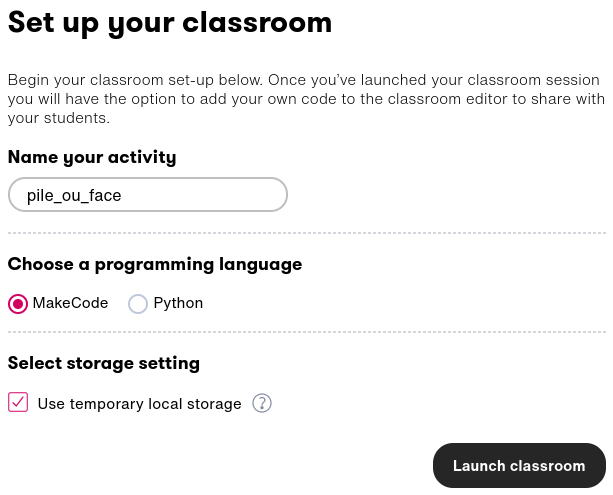
\includegraphics[width=0.7\linewidth]{res/classroom_setup2.png}}~\\
\end{methode}

\begin{remarque}
    Il est possibe de choisir si l'on souhaite autoriser l'application à enregistrer des données
     localement (dans le "local storage" du navigateur), à éviter si l'ordinateur est partagé 
     mais utile si l'on craint de perdre son travail.
\end{remarque}
\vspace{5mm}

\subsubsection{Proposer un programme}


\begin{methode}
    Dans le bandeau supérieur on trouve le menu de ce qui correspond aux 4 étapes
     de la vie d'une session :
     \begin{enumerate}
        \item Création du code dans l'éditeur.
        \item Partage de la session.
        \item Supervision des travaux.
        \item Sauvegarde et clôture d'une session.
     \end{enumerate}~\\

    \centerline{
\includegraphics[width=0.8\linewidth]{res/classroom_menu.png}}
    
    Il faut donc commencer par ouvrir l'éditeur (ici pour la programmation en blocs) et écrire
    un programme ou un début de programme (par exemple celui proposé par la fiche "pile ou face").
    \vspace{5mm}

    \centerline{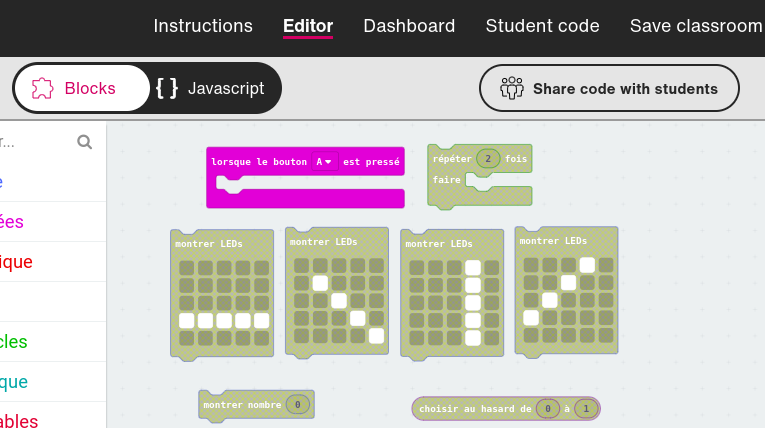
\includegraphics[width=0.6\linewidth]{res/classroom_editor.png}}~\\

    Une fois le code terminé, il ne faut pas oublier de le partager en cliquant sur le bouton
     "Share code with students".

\end{methode}


\begin{remarque}
    L'éditeur comporte les mêmes fonctionnalités que sur \url{http://makecode.microbit.org}, il est donc possible de :
    \begin{itemize}
        \item télécharger le code.
        \item appairer la carte \mb avec le navigateur.
        \item ouvrir un programme compilé sous la forme d'un fichier .hex en faisant glisser ce fichier
        dans la fenêtre de classroom.
        
    \end{itemize}
    
    Le code peut être modifié ultérieurement pour être distribué à toute la classe ou de façon ciblée,
     ce qui permet un travail de différenciation.
 
\end{remarque}

\vspace{5mm}

\subsubsection{Partager la session}

\begin{methode}
    Pour se connecter à la session, les élèves doivent aller sur le site :  \url{http://microbit.org/join}
     renseigner le nom de la classe (l'occasion de réviser son vocabulaire anglais)
    et rentrer le code PIN.
    \vspace{5mm}

    \centerline{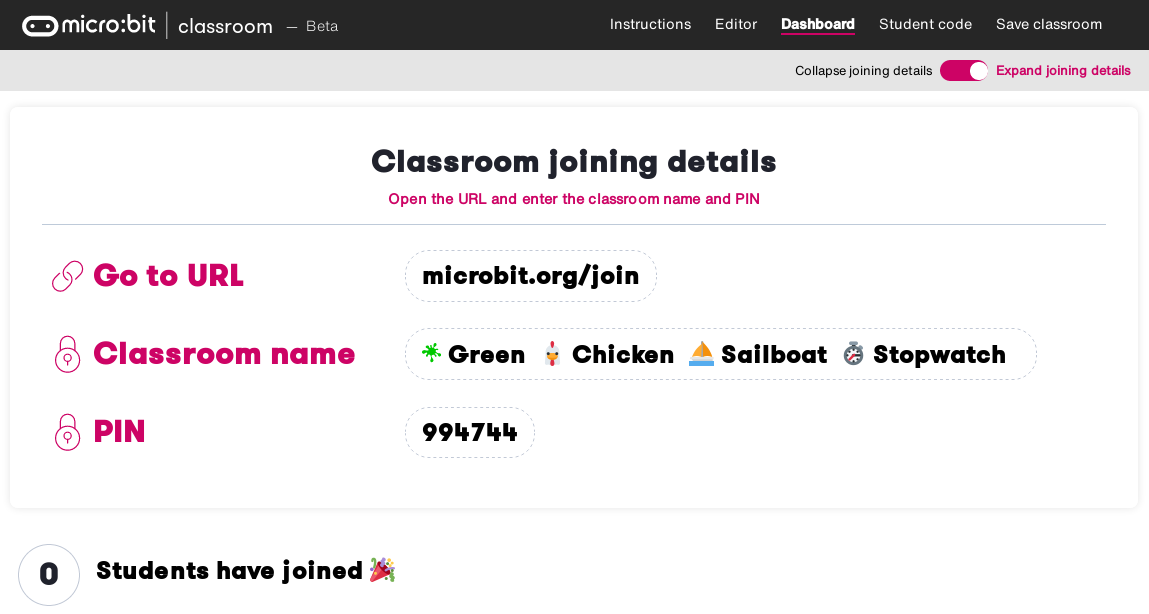
\includegraphics[width=0.7\linewidth]{res/classroom_dashboard2.png}}
    
\end{methode}


\newpage
\vspace{5mm}~\\

\begin{remarque}
    Une fois connectés, les élèves renseigneront leur nom tel qu'il apparaîtra sur votre écran,
    mais aussi tel qu'il sera enregistré dans le fichier de sauvegarde et de compte-rendu, attention
    aux noms fantaisistes.
    
\end{remarque}

\vspace{5mm}

\subsubsection{Superviser les travaux}

\begin{methode}
        Dans cette fenêtre, la liste des élèves apparaît à gauche avec l'indication 
        de l'état de son travail : en cours ou terminé (avec en prime une autoévaluation sous la
        forme de smiley).\\
        Dans la partie droite apparait le travail de l'élève dont les modifications sont instantannément
        reportées. Là encore on retrouve le bouton "Share code with students" qui permet d'envoyer à tout
        ou une partie de la classe le code produit par un élève.

    \vspace{5mm}
    
    \centerline{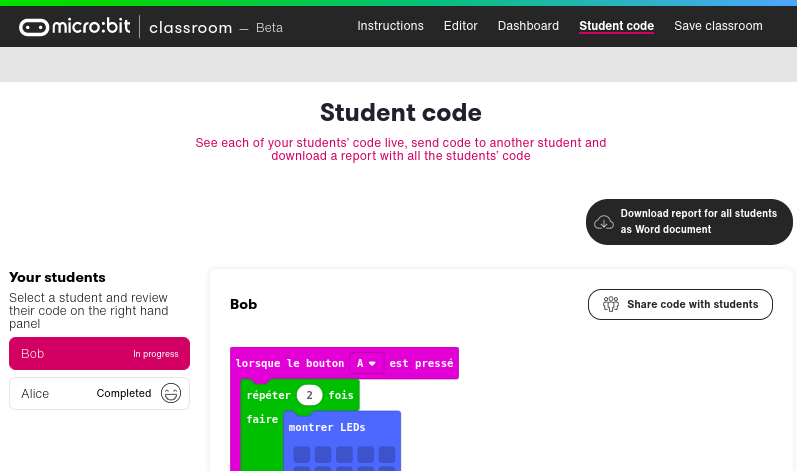
\includegraphics[width=0.6\linewidth]{res/classroom_studentCode2.png}}
    


\end{methode}

\begin{remarque}
    Pour l'éditeur de programmation par bloc, seul les blocs actifs côté élève
    apparaitront dans la fenêtre de supervision.
    
\end{remarque}


\newpage
\vspace{5mm}~\\

\subsubsection{Sauvegarder une session}

    \begin{methode}
        Cette dernière étape de la vie d'une session vous permettra de récupérer un fichier html
        contenant toutes les informations nécessaires pour reprendre le travail ultérieurement.
        Le fait de clôturer la session, rendra inactive la connexion.
        
    \vspace{5mm}
    
    \centerline{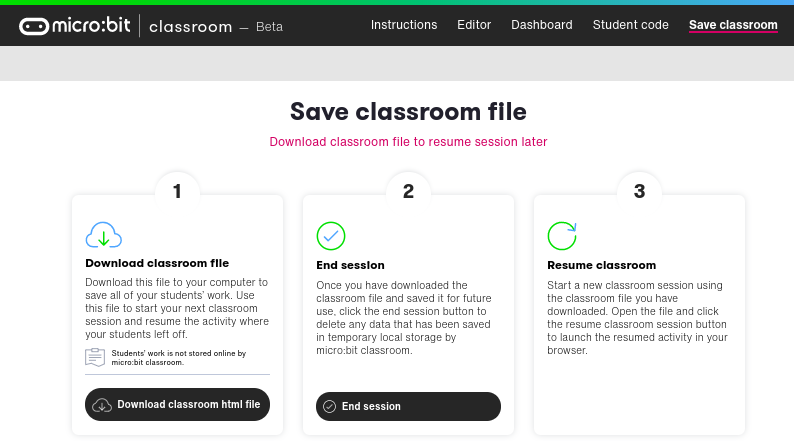
\includegraphics[width=0.7\linewidth]{res/classroom_save.png}}
        
        Pour reprendre le travail, il suffit d'ouvrir fichier .html dans le navigateur et l'on 
        retrouvera le dernier programme proposé ainsi que les travaux des élèves. Ils pourront
         dès lors de nouveau se connecter, et sélectionner leur nom dans un menu déroulant afin de 
         retrouver leur travail.

    \end{methode}

    \begin{remarque}
        Attention au paramètrage du navigateur, si celui est trop strict sur la gestion des
         données personnelles vous pourriez être dans l'impossibilité de réouvrir correctement
         une session.
    \end{remarque}

